\vspace{-0.5em}
\section{Introduction}
\vspace{-0.5em}

Language model (LM) based agents are rapidly improving, and are now able to tackle digital tasks such as navigating the web \citep{zhou2024webarena,deng2023mindweb} or operating mobile apps \citep{rawles2023androidinthewild,rawles2024androidworld}. 
Current agents mostly integrate a fixed set of given examples via training \citep{fu2024autoguide,murty2024bagel} or in-context learning \citep{zheng2024synapse}. This allows them to perform well on action sequences similar to those presented in these examples, but results in a lack of robustness to changes in task contexts or environments \citep{deng2023mindweb}. Essentially, they fail to grasp the key to disentangling increasingly complex tasks --- to extract and learn reusable task workflows shared across similar tasks and environments \citep{yu2023language,wang2024voyager}. 
Moreover, as agents solve each task separately, they do not learn from past successes and failures, and are therefore unable to adapt over time \citep{yoran2024assistantbench}.



\begin{wrapfigure}[16]{r}{0.6\textwidth}
\vspace{-6mm}
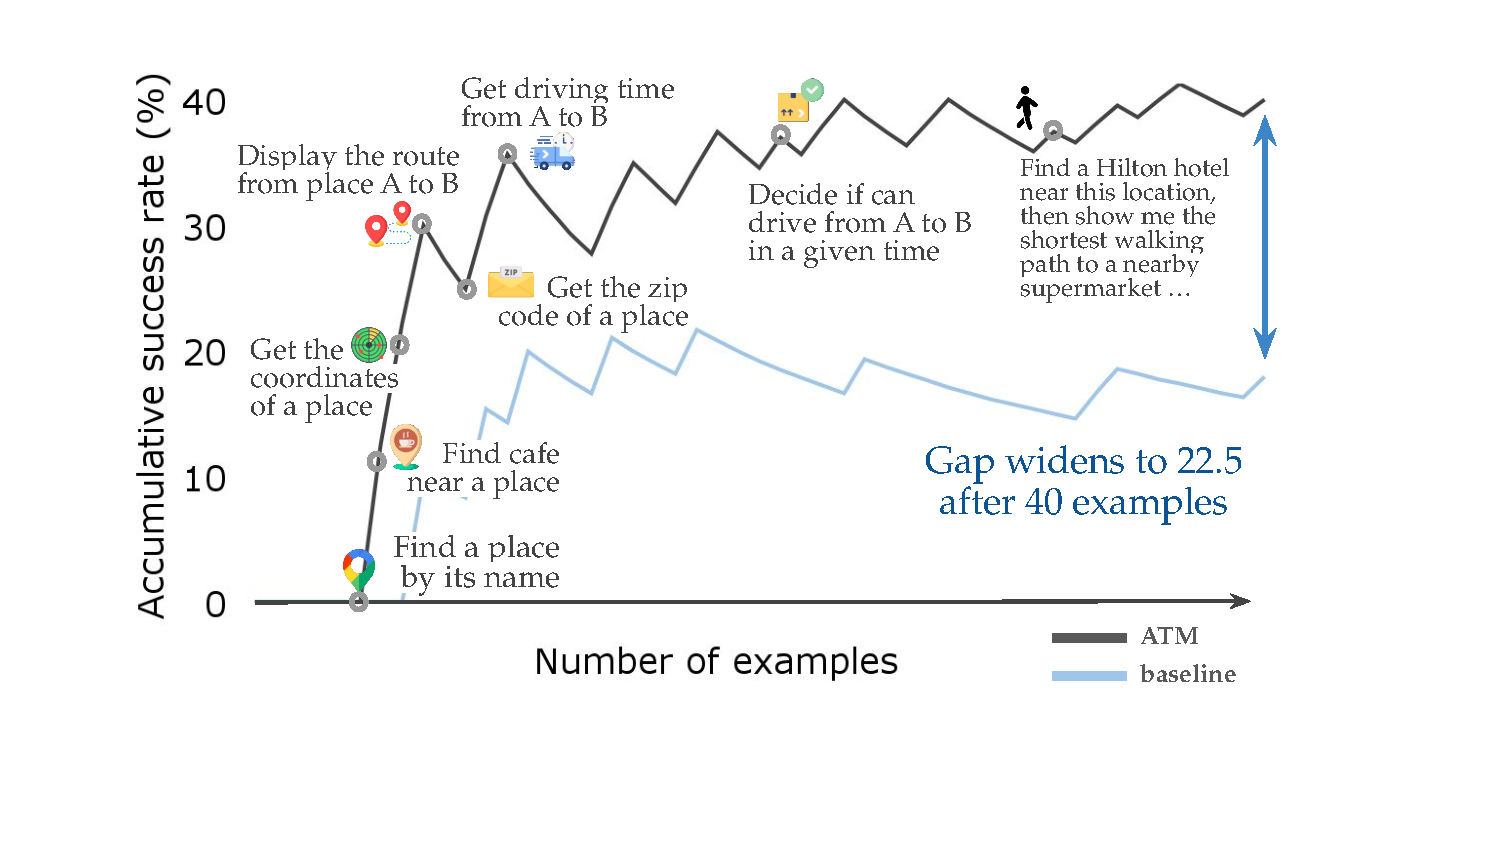
\includegraphics[width=0.59\textwidth]{./figures/teaser.pdf}
\vspace{-3mm}
\caption{\awm enables agents to continuously induce and apply workflows to improve performance, compared to stagnant baselines. We show results by \awm on the WebArena map split as an example.}
\label{fig:teaser}
\vspace{3mm}
\end{wrapfigure}


Motivated by how humans abstract common task routines from past experiences and apply such knowledge to guide future activities \citep{chi1981categorization,chi2014nature}, we propose agent workflow memory (\awm) (\S\ref{sec:3:method}) to realize a similar mechanism in agents. \awm induces workflows from agent trajectories by extracting reusable routines, and then integrates these workflows into agent memory to guide future task-solving processes. Each workflow represents a goal with a common routine extracted from available action trajectories, which allows it to effectively capture the most essential and reusable skills agents need to acquire to successfully solve increasingly complex tasks.
%
As an example, \autoref{fig:teaser} shows workflows induced by \awm on the WebArena map test split of the  benchmark \citep{zhou2024webarena}.
\awm starts with a basic set of built-in actions and solves new tasks in a streaming manner, continuously inducing workflows from the task at hand, \eg, learning to ``find a place by its name'' from the first few examples. Moreover, \awm continues to build more complex workflows on top of new experiences and previously acquired workflows. 
For example, the  ``find a place by its name'' workflow, once induced, effectively serves as a subgoal to build a more complex workflow ``get the zip code of a place.'' 
%
Such continual learning mechanisms create a snowball effect to induce and apply increasingly complex workflows while expanding the agent memory, often yielding a substantial performance gap over a vanilla agent that does not adapt. This gap over the baseline rises as high as $22.5$ points on WebArena after rolling over only tens of examples (as shown by \autoref{fig:teaser}).

\awm readily operates in both \textit{offline} and \textit{online} scenarios, where annotated examples are either available or non-existent. When high-quality annotated examples are available for a task, \awm operating in an \textit{offline} fashion can extract reusable workflows from these canonical examples and integrate them into memory to assist test-time inference. Even if no annotated examples exist, \awm \textit{online} can also run in an \textit{supervision-free setting}, where it iteratively induces workflows from self-generated past predictions that are judged correct by an evaluator module.


We evaluate \awm on two agent web navigation benchmarks (\S\ref{sec:4:experiments}): WebArena, which provides rigorous execution-based evaluation \citep{zhou2024webarena}, and Mind2Web, which emphasizes broad tasks and domain coverage \citep{deng2023mindweb}.
On WebArena, \awm improves over the top published autonomous method \citep{drouin2024workarena} by $51.1$\% relative success rate, and even outperforms methods augmented with human expert written workflows \citep{sodhi2023heap} by $7.9$\%.
On Mind2Web, \awm effectively improves the cross-task results by $24.6$\% in relative step-wise success rate. 
% Results on both benchmarks demonstrate the substantial effect of \awm in solving tasks more successfully.

We further demonstrate the generalizability of \awm on both datasets.
On WebArena, we create a cross-template subset where each example is instantiated from different task templates. \awm still consistently surpasses all baseline approaches, demonstrating its reliable cross-task workflow adaptability (\S\ref{sec:4.1:webarena}).
On Mind2Web, we evaluate \awm on the cross-website and cross-domain test splits to examine its domain generality, where it scores $8.9$--$14.0$ absolute points higher over baseline, and the margins become more substantial as the train-test distribution gap widens (\S\ref{sec:4.2:mind2web}). Both results show the superior generalization of \awm across tasks, websites, and domains.

% Beyond augmenting agent memory with induced workflows, we further experiment with expanding the agent action space by transforming workflows into executable actions. Our results show the auxiliary benefit of extending the actions space, yet our case studies reveal the need for more advances, such as providing intermediate environment access and dynamic workflow execution loops (\S\ref{sec:expand-action}).
% Overall, we hope our \awm approach demonstrates a promising direction to improve and adapt digital agents, and inspires more work throughout workflow induction and integration.